\begin{figure}
    \centering
    \resizebox{\textwidth}{!}{%
    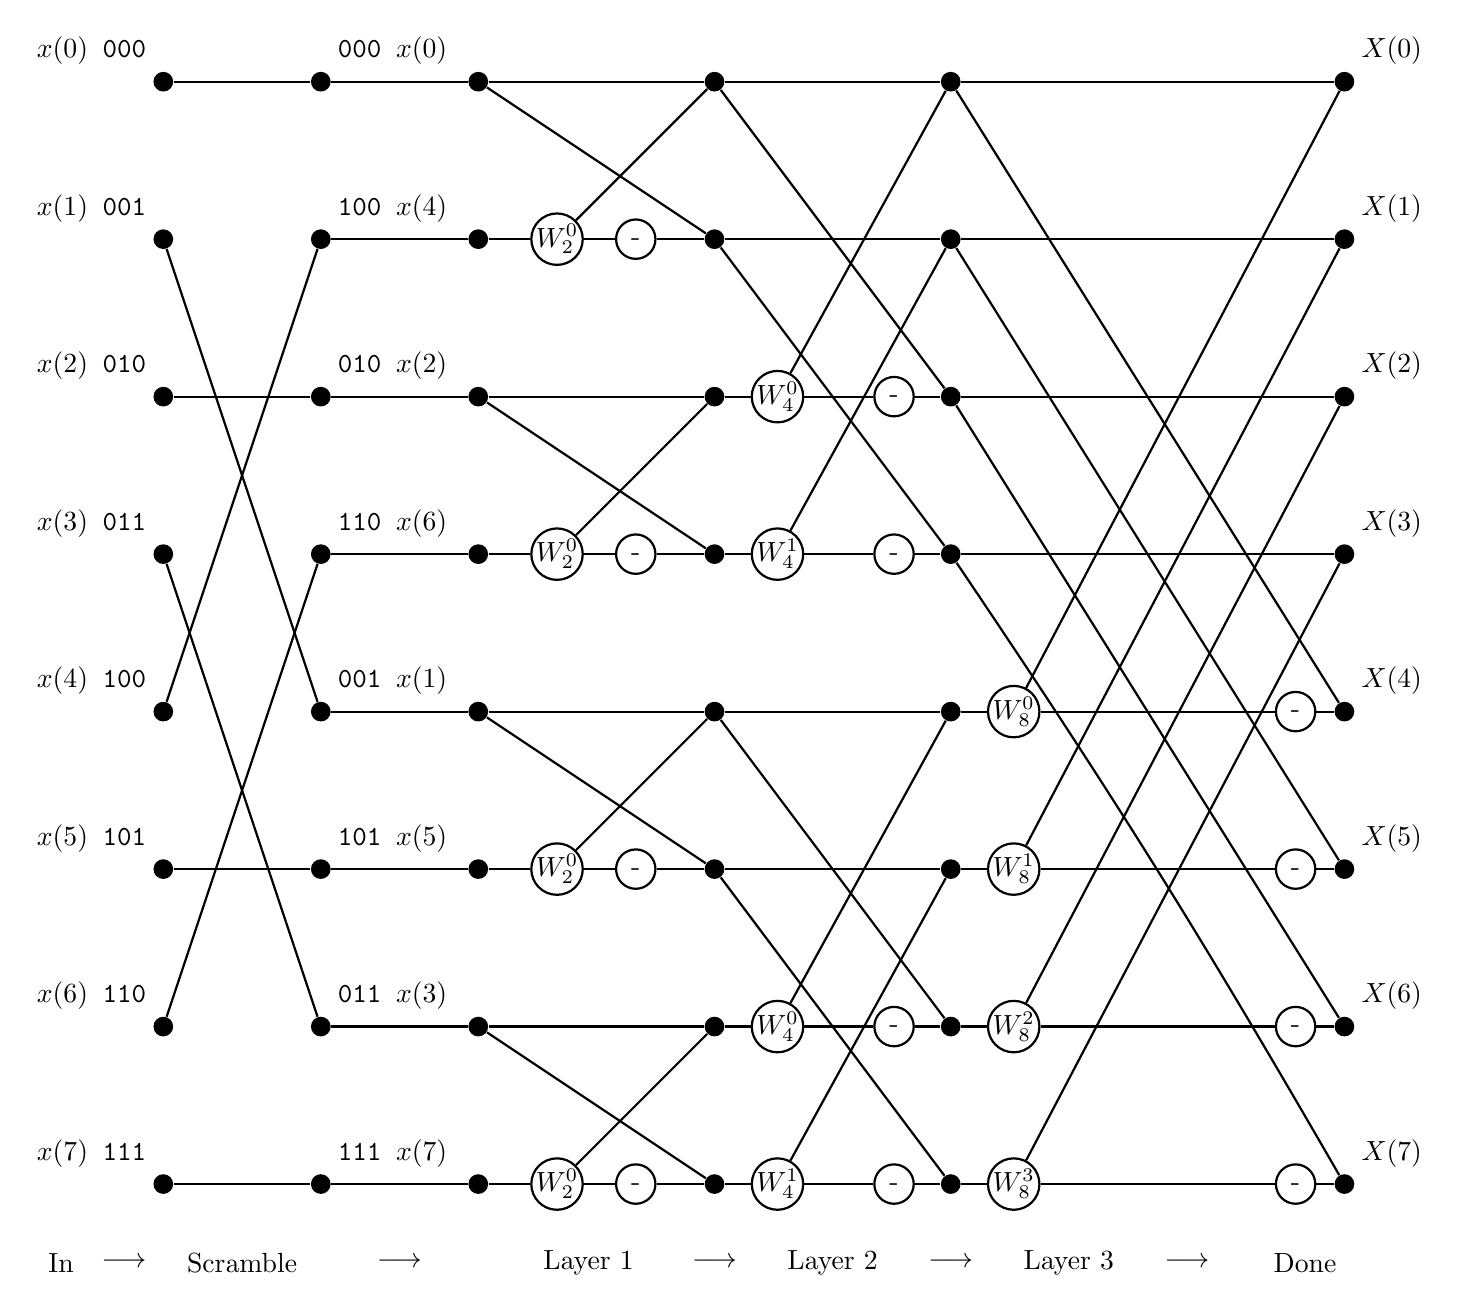
\begin{tikzpicture}[
        dot/.style = {circle, fill, inner sep = 0mm, minimum size = 2.5mm},
        op/.style = {draw, thick, circle, inner sep = 0mm, minimum size = 5mm},
        func/.style = {draw, thick, circle, inner sep = 1mm},
        arr/.style = {draw, thick},
    ]
        \node (in0) at (0, 14) [dot, label=above left:$x(0)$\texttt{ 000}]{};
        \node (in1) at (0, 12) [dot, label=above left:$x(1)$\texttt{ 001}]{};
        \node (in2) at (0, 10) [dot, label=above left:$x(2)$\texttt{ 010}]{};
        \node (in3) at (0,  8) [dot, label=above left:$x(3)$\texttt{ 011}]{};
        \node (in4) at (0,  6) [dot, label=above left:$x(4)$\texttt{ 100}]{};
        \node (in5) at (0,  4) [dot, label=above left:$x(5)$\texttt{ 101}]{};
        \node (in6) at (0,  2) [dot, label=above left:$x(6)$\texttt{ 110}]{};
        \node (in7) at (0,  0) [dot, label=above left:$x(7)$\texttt{ 111}]{};

        \node (sc0) at (2, 14) [dot, label=above right:\texttt{000 }$x(0)$]{};
        \node (sc4) at (2, 12) [dot, label=above right:\texttt{100 }$x(4)$]{};
        \node (sc2) at (2, 10) [dot, label=above right:\texttt{010 }$x(2)$]{};
        \node (sc6) at (2,  8) [dot, label=above right:\texttt{110 }$x(6)$]{};
        \node (sc1) at (2,  6) [dot, label=above right:\texttt{001 }$x(1)$]{};
        \node (sc5) at (2,  4) [dot, label=above right:\texttt{101 }$x(5)$]{};
        \node (sc3) at (2,  2) [dot, label=above right:\texttt{011 }$x(3)$]{};
        \node (sc7) at (2,  0) [dot, label=above right:\texttt{111 }$x(7)$]{};

        \path[arr] (in0) -- (sc0);
        \path[arr] (in1) -- (sc1);
        \path[arr] (in2) -- (sc2);
        \path[arr] (in3) -- (sc3);
        \path[arr] (in4) -- (sc4);
        \path[arr] (in5) -- (sc5);
        \path[arr] (in6) -- (sc6);
        \path[arr] (in7) -- (sc7);

        \node (l00) at (4, 14) [dot]{};
        \node (l01) at (4, 12) [dot]{};
        \node (l02) at (4, 10) [dot]{};
        \node (l03) at (4,  8) [dot]{};
        \node (l04) at (4,  6) [dot]{};
        \node (l05) at (4,  4) [dot]{};
        \node (l06) at (4,  2) [dot]{};
        \node (l07) at (4,  0) [dot]{};

        \path[arr] (sc0) -- (l00);
        \path[arr] (sc4) -- (l01);
        \path[arr] (sc2) -- (l02);
        \path[arr] (sc6) -- (l03);
        \path[arr] (sc1) -- (l04);
        \path[arr] (sc5) -- (l05);
        \path[arr] (sc3) -- (l06);
        \path[arr] (sc7) -- (l07);

        \node (w01) at (5, 12) [op]{$W_2^0$};
        \node (w03) at (5,  8) [op]{$W_2^0$};
        \node (w05) at (5,  4) [op]{$W_2^0$};
        \node (w07) at (5,  0) [op]{$W_2^0$};

        \node (m01) at (6, 12) [op]{-};
        \node (m03) at (6,  8) [op]{-};
        \node (m05) at (6,  4) [op]{-};
        \node (m07) at (6,  0) [op]{-};

        \node (l10) at (7, 14) [dot]{};
        \node (l11) at (7, 12) [dot]{};
        \node (l12) at (7, 10) [dot]{};
        \node (l13) at (7,  8) [dot]{};
        \node (l14) at (7,  6) [dot]{};
        \node (l15) at (7,  4) [dot]{};
        \node (l16) at (7,  2) [dot]{};
        \node (l17) at (7,  0) [dot]{};

        \path[arr] (l01) -- (w01);
        \path[arr] (l03) -- (w03);
        \path[arr] (l05) -- (w05);
        \path[arr] (l07) -- (w07);
        \path[arr] (w01) -- (m01);
        \path[arr] (w03) -- (m03);
        \path[arr] (w05) -- (m05);
        \path[arr] (w07) -- (m07);
        \path[arr] (m01) -- (l11);
        \path[arr] (m03) -- (l13);
        \path[arr] (m05) -- (l15);
        \path[arr] (m07) -- (l17);

        \path[arr] (w01) -- (l10);
        \path[arr] (w03) -- (l12);
        \path[arr] (w05) -- (l14);
        \path[arr] (w07) -- (l16);
        \path[arr] (l00) -- (l10);
        \path[arr] (l02) -- (l12);
        \path[arr] (l04) -- (l14);
        \path[arr] (l06) -- (l16);
        \path[arr] (l00) -- (l11);
        \path[arr] (l02) -- (l13);
        \path[arr] (l04) -- (l15);
        \path[arr] (l06) -- (l17);

        \node (w12) at (7.8, 10) [op]{$W_4^0$};
        \node (w13) at (7.8,  8) [op]{$W_4^1$};
        \node (w16) at (7.8,  2) [op]{$W_4^0$};
        \node (w17) at (7.8,  0) [op]{$W_4^1$};

        \node (m12) at (9.28, 10) [op]{-};
        \node (m13) at (9.28,  8) [op]{-};
        \node (m16) at (9.28,  2) [op]{-};
        \node (m17) at (9.28,  0) [op]{-};

        \node (l20) at (10, 14) [dot]{};
        \node (l21) at (10, 12) [dot]{};
        \node (l22) at (10, 10) [dot]{};
        \node (l23) at (10,  8) [dot]{};
        \node (l24) at (10,  6) [dot]{};
        \node (l25) at (10,  4) [dot]{};
        \node (l26) at (10,  2) [dot]{};
        \node (l27) at (10,  0) [dot]{};

        \path[arr] (l10) -- (l20);
        \path[arr] (l10) -- (l22);
        \path[arr] (l11) -- (l21);
        \path[arr] (l11) -- (l23);
        \path[arr] (l14) -- (l24);
        \path[arr] (l14) -- (l26);
        \path[arr] (l15) -- (l25);
        \path[arr] (l15) -- (l27);

        \path[arr] (w12) -- (l20);
        \path[arr] (w13) -- (l21);
        \path[arr] (w16) -- (l24);
        \path[arr] (w17) -- (l25);

        \path[arr] (l12) -- (w12);
        \path[arr] (l13) -- (w13);
        \path[arr] (l16) -- (w16);
        \path[arr] (l17) -- (w17);

        \path[arr] (w12) -- (m12);
        \path[arr] (w13) -- (m13);
        \path[arr] (w16) -- (m16);
        \path[arr] (w17) -- (m17);

        \path[arr] (m12) -- (l22);
        \path[arr] (m13) -- (l23);
        \path[arr] (m16) -- (l26);
        \path[arr] (m17) -- (l27);

        \node (l30) at (15, 14) [dot, label=above right:$X(0)$]{};
        \node (l31) at (15, 12) [dot, label=above right:$X(1)$]{};
        \node (l32) at (15, 10) [dot, label=above right:$X(2)$]{};
        \node (l33) at (15,  8) [dot, label=above right:$X(3)$]{};
        \node (l34) at (15,  6) [dot, label=above right:$X(4)$]{};
        \node (l35) at (15,  4) [dot, label=above right:$X(5)$]{};
        \node (l36) at (15,  2) [dot, label=above right:$X(6)$]{};
        \node (l37) at (15,  0) [dot, label=above right:$X(7)$]{};

        \node (w24) at (10.8, 6) [op]{$W_8^0$};
        \node (w25) at (10.8, 4) [op]{$W_8^1$};
        \node (w26) at (10.8, 2) [op]{$W_8^2$};
        \node (w27) at (10.8, 0) [op]{$W_8^3$};

        \path[arr] (w24) -- (l30);
        \path[arr] (w25) -- (l31);
        \path[arr] (w26) -- (l32);
        \path[arr] (w27) -- (l33);

        \node (m24) at (14.38, 6) [op, fill=white]{-};
        \node (m25) at (14.38, 4) [op, fill=white]{-};
        \node (m26) at (14.38, 2) [op, fill=white]{-};
        \node (m27) at (14.38, 0) [op, fill=white]{-};

        \path[arr] (l24) -- (w24);
        \path[arr] (w24) -- (m24);
        \path[arr] (m24) -- (l34);
        \path[arr] (l25) -- (w25);
        \path[arr] (w25) -- (m25);
        \path[arr] (m25) -- (l35);
        \path[arr] (l26) -- (w26);
        \path[arr] (w26) -- (m26);
        \path[arr] (m26) -- (l36);
        \path[arr] (l27) -- (w27);
        \path[arr] (w27) -- (m27);
        \path[arr] (m27) -- (l37);

        \path[arr] (l20) -> (l30);
        \path[arr] (l21) -> (l31);
        \path[arr] (l22) -> (l32);
        \path[arr] (l23) -> (l33);
        \path[arr] (l20) -> (l34);
        \path[arr] (l21) -> (l35);
        \path[arr] (l22) -> (l36);
        \path[arr] (l23) to[bend left=2] (l37);

        \node at (-1.3, -1) {In};
        \node at (-0.5, -1) {$\longrightarrow$};
        \node at (1, -1) {Scramble};
        \node at (3, -1) {$\longrightarrow$};
        \node at (5.4, -1) {Layer 1};
        \node at (7, -1) {$\longrightarrow$};
        \node at (8.5, -1) {Layer 2};
        \node at (10, -1) {$\longrightarrow$};
        \node at (11.5, -1) {Layer 3};
        \node at (13, -1) {$\longrightarrow$};
        \node at (14.5, -1) {Done};
    \end{tikzpicture}
    }%
    \caption{Example datapath representation of in-place FFT algorithm with $N = 8$.
    \label{fig:lattice}}
\end{figure}
